\documentclass[11pt,a4paper]{article}
\usepackage[margin=2.5cm]{geometry}
\usepackage{booktabs}
\usepackage{graphicx}
\usepackage{xcolor}
\usepackage{hyperref}
\usepackage{enumitem}
\usepackage{titlesec}
\usepackage{fancyhdr}
\usepackage{microtype}
\usepackage{parskip}
\usepackage{fontspec}
\usepackage{polyglossia}
\usepackage{amsmath}
\usepackage{amssymb}

\setmainlanguage{english}
\setotherlanguage{hebrew}
\newfontfamily\hebrewfont{DejaVu Sans}[Script=Hebrew]

\hypersetup{colorlinks=true, linkcolor=blue, urlcolor=blue}

\pagestyle{fancy}
\fancyhf{}
\rhead{Knesset Protocol Journal Project}
\lhead{Step 7 --- Gold Evaluation}
\rfoot{Page \thepage}
\lfoot{Tomer Morad, Or Israeli, Yoel Marko --- July 2026}

\titleformat{\section}{\large\bfseries}{\thesection.}{0.6em}{}[\titlerule]
\titleformat{\subsection}{\normalsize\bfseries}{\thesubsection}{0.6em}{}

\begin{document}

\begin{center}
  {\LARGE \textbf{Gold Evaluation \& Re-Validation}}\\[0.3em]
  {\large Step 7 --- Do Steps 2--5's marker-based findings hold up on real gold?}\\[0.6em]
  {\normalsize Tomer Morad \quad Or Israeli \quad Yoel Marko}\\
  {\normalsize July 2026}
\end{center}

\vspace{0.5em}

\section{Objective}

Steps 2--5 evaluated Task~1 (clustering) and Task~2 (linking) against \emph{marker-derived}
canonical topics (151 topics, only 30 recurring) --- a proxy for gold, not gold itself. Step~6
produced real full-protocol gold segmentation (523 segments, 211/213 protocols). This step
converts that into gold data for both tasks and re-runs every prior evaluation against it, to
check whether the earlier conclusions (best representation, best hybrid weight, expected
streaming performance) actually hold at realistic granularity.

\section{Method}

\texttt{build\_gold.py} converts \texttt{segmentation.json} into \texttt{gold\_segments.json}
(523 segments) and \texttt{gold\_chains.json} (topic string $\to$ chronological occurrence
list; 22 keys have $\ge 2$ occurrences $=$ recurring). \texttt{embed\_gold.py} computes e5 and
AlephBERT embeddings of every gold span on GPU. \texttt{gold\_reeval.py} re-runs Task~1
clustering (ARI/AUC) and Task~2 pairwise + streaming linking (precision/recall/F1) against this
gold, exactly mirroring Steps 3--5's methodology. \texttt{gold\_abtt\_and\_hybrid.py}
re-sweeps ABTT $k$ and the hybrid $\alpha$ weight to check whether Step 3--4's tuned values
still hold.

\section{Results}

\subsection{Task 1 --- Clustering (58 recurring gold segments, 22 gold topics)}
\begin{center}
\begin{tabular}{lrrr}
\toprule
\textbf{Representation} & \textbf{ARI (agglom.)} & \textbf{ARI (kmeans)} & \textbf{AUC} \\
\midrule
TF-IDF & 0.382 & 0.407 & 0.874 \\
\textbf{e5\_k1} & \textbf{0.657} & \textbf{0.515} & \textbf{0.954} \\
AlephBERT $k{=}2$ & 0.265 & 0.274 & 0.854 \\
Hybrid $\alpha{=}0.6$ & 0.265 (spectral 0.411) & --- & 0.884 \\
\bottomrule
\end{tabular}
\end{center}

\subsection{Task 2 --- Linking}
Pairwise (oracle): e5\_k1 best F1$=0.62$ @ $\theta{=}0.26$, AUC$=0.954$ --- all higher than the
Step 3/5 marker-based estimates.

\textbf{Streaming (realistic) --- the headline result:}
\begin{center}
\begin{tabular}{lrrr}
\toprule
\textbf{Representation} & \textbf{Best F1} & \textbf{Precision at that point} & \textbf{Recall} \\
\midrule
e5\_k1 & 0.125 & 7.7\% & 33\% \\
AlephBERT $k{=}2$ & 0.075 & 4.2\% & 33\% \\
Hybrid $\alpha{=}0.6$ & 0.090 & 5.2\% & 33\% \\
\bottomrule
\end{tabular}
\end{center}

Streaming F1 collapsed from Step 5's marker-based estimate of 0.41 to 0.125 on real gold. At
the best threshold, roughly 92\% of ``LINK'' predictions are false merges.

\begin{center}
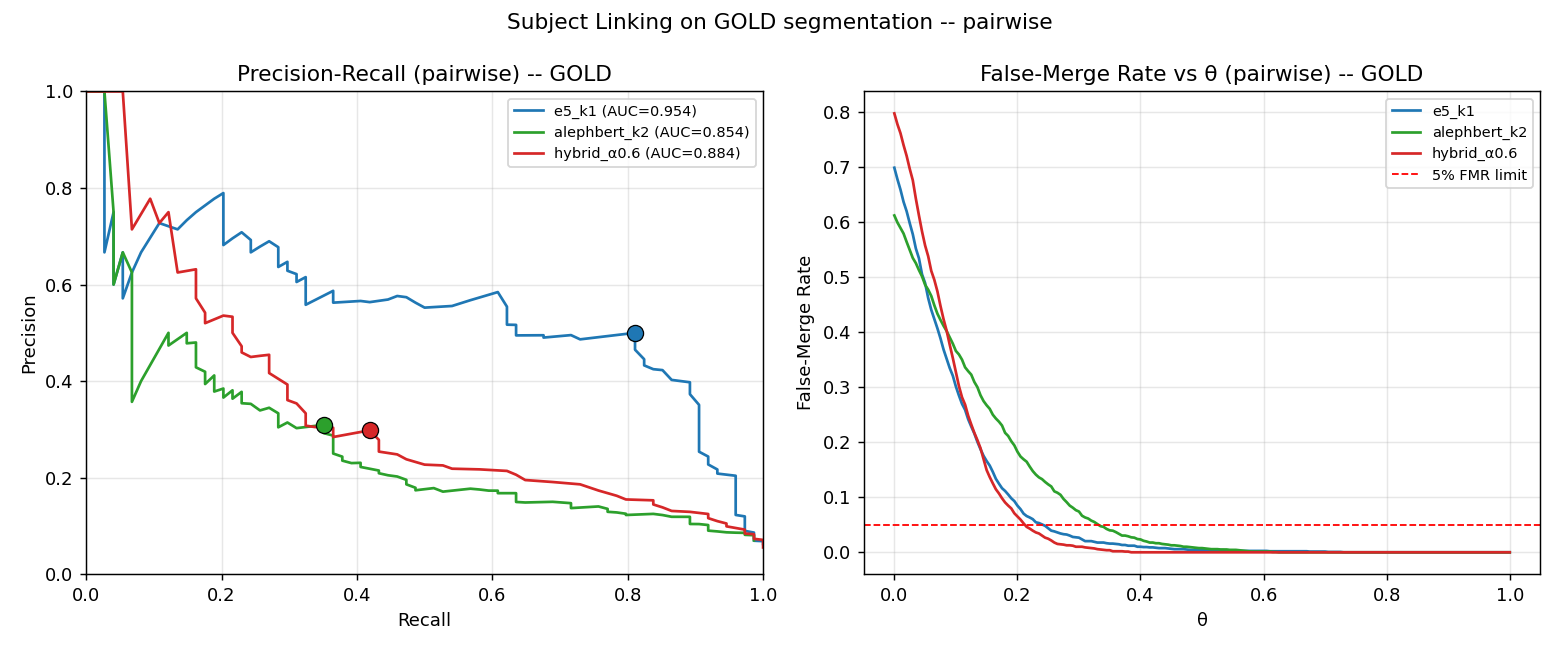
\includegraphics[width=0.48\textwidth]{../outputs/gold_pr_curves_pairwise.png}
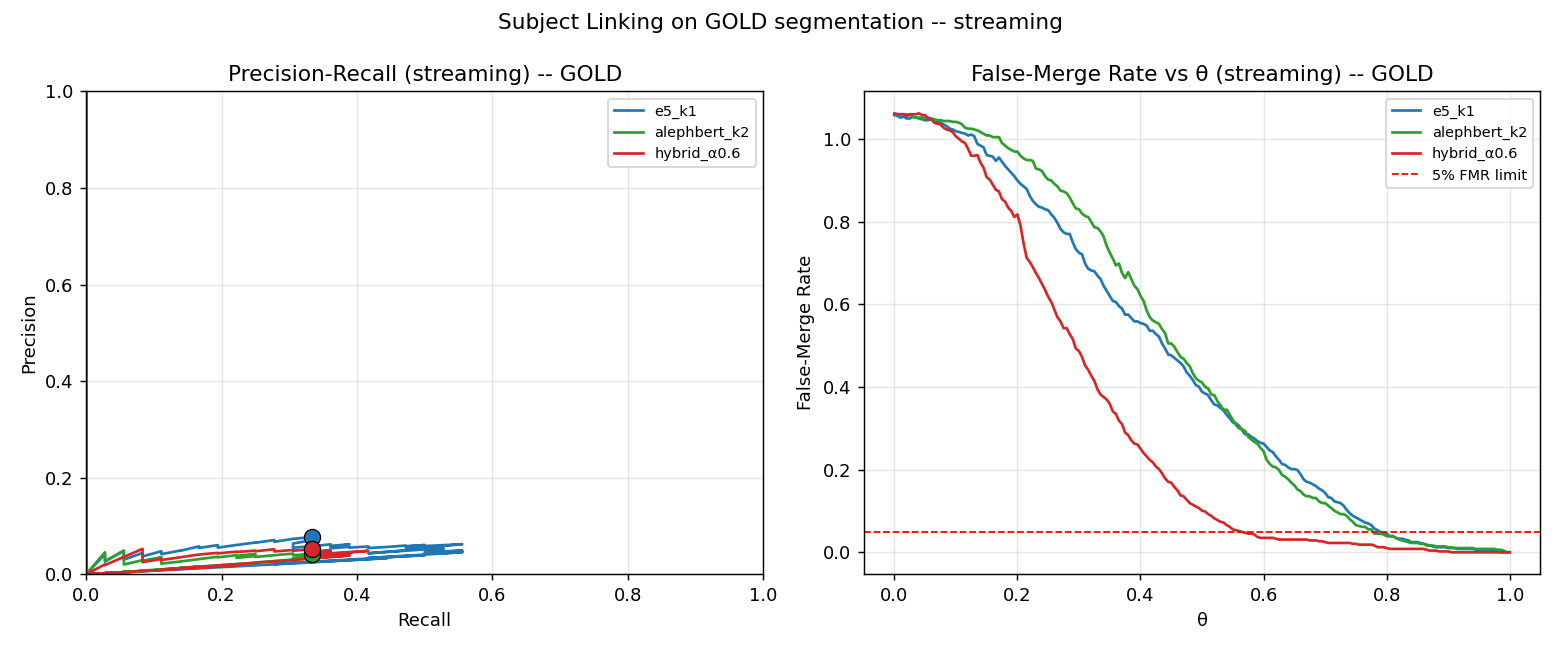
\includegraphics[width=0.48\textwidth]{../outputs/gold_pr_curves_streaming.png}
\end{center}

\section{Key Finding}

\textbf{Not a representation problem.} e5\_k1 is still the best representation tried, by an even
wider margin than on marker-based data. \textbf{It is a task-formulation problem:} gold
segmentation is far more fine-grained (523 segments, only 22 ever recur) than the old canonical
topics (30/151 recurring), so true ``same subject'' pairs are rare, and any similarity threshold
loose enough to catch them is loose enough to flood in unrelated same-sounding topics. No fixed
cosine cutoff can be both loose enough for recall and tight enough for precision at this
granularity.

Follow-up checks ruled out easy fixes: Step 4's hybrid finding does not replicate on gold
(hybrid is worse than plain e5\_k1 on every clustering metric), and re-sweeping ABTT $k$
confirms e5 $k{=}1$ is still $\approx$optimal.

\section{What Needs Improvement}

\begin{enumerate}[leftmargin=1.4em]
  \item \textbf{The core open problem}: no embedding-threshold method can fix the precision
        ceiling demonstrated here. This directly motivated Step 8 (retrieve-then-verify with
        an LLM), which is itself still below this baseline as of writing --- see that report.
  \item \textbf{No representation tuning left to try.} e5\_k1 unchanged is confirmed as the
        representation to carry forward; further ABTT/hybrid sweeps are not expected to help.
  \item \textbf{Gold chain undercount.} As noted in Step 6, no label canonicalization was
        applied, so the ``22 recurring topics'' figure is likely an undercount of true
        recurrence in the corpus --- some real repeats are hidden as singleton chains under
        slightly different generated labels.
\end{enumerate}

\vspace{1.5em}
\hrule
\vspace{0.4em}
\raggedright
{\small
\textbf{Artifacts (this step):} \newline
\texttt{outputs/gold\_segments.json}, \texttt{outputs/gold\_chains.json}, \newline
\texttt{outputs/gold\_reeval\_results.json}, \texttt{outputs/gold\_abtt\_sweep.json}, \newline
\texttt{outputs/gold\_hybrid\_clustering.json}, \texttt{outputs/embeddings/} \newline
\textbf{Code:} \texttt{code/build\_gold.py}, \texttt{code/embed\_gold.py},
\texttt{code/gold\_reeval.py}, \texttt{code/gold\_abtt\_and\_hybrid.py}.
}

\end{document}
